\chapter{Bayesian Statistics and Markov Chain Monte Carlo Techniques}
\label{chap:MarkovChainMonteCarlo}
This thesis presents a Bayesian oscillation analysis. To extract the oscillation parameters, a Markov Chain Monte Carlo (MCMC) method is used. This chapter explains the theory of how parameter estimates can be determined using this technique and condenses the material found in the literature \cite{mcmc_handbook, mcmc_practice, thesis_clarence, thesis_kirsty}.

The oscillation parameter determination presented within this thesis is built upon a simultaneous fit to neutrino beam data in the near detector, beam data at SK and atmospheric data at SK. In total, there are four oscillation parameters of interest (\sinsqatm, \sinsqreac, \delmsqatm, and \dcp), two oscillation parameters to which this study will not be sensitive (\sinsqsol, \delmsqsol) and  many nuisance parameters that control the systematic uncertainty models invoked within this study.
%The systematic uncertainties can be grouped into categories depending on how they are defined: $574$ bin-normalisations due to the near detector response, $45$ bin-normalisations to describe the far detector response to neutrino beam events, $27$ parameters to describe the detector response to atmospheric neutrino events, $100$ to model the bin-normalisation due to beam flux uncertainties, $18$ which model the atmospheric flux uncertainties, and $87$ to describe the correlated cross-section model. An alternative parameterisation, where the far detector response is correlated between the beam and atmospheric samples, replaces the bin-normalisation parameters with $224$ shift and smear systematics. Section Link to Systematics Chapter describes the systematic model in more depth.

The MCMC technique generates a multi-dimensional probability distribution across all of the model parameters used in the fit. To determine the parameter estimate of a single parameter, this multi-dimensional object is integrated over all other parameters. This process is called Marginalisation and is further described in \autoref{sec:MarkovChainMonteCarlo_Marginalisation}. Monte Carlo techniques approximate the probability distribution of each parameter within the limit of generating infinite samples. As ever, generating a large number of samples is time and resource-dependent. Therefore, an MCMC technique is utilised within this analysis to reduce the required number of steps to sufficiently sample the parameter space. This technique is described in further detail in \autoref{sec:MarkovChainMonteCarlo_MarkovChainMC}.

\section{Bayesian Statistics}
\label{sec:MarkovChainMonteCarlo_BayesianStatistics}

Bayesian inference treats observable data, \quickmath{D}, and model parameters, \quickmath{\vec{\theta}}, on equal footing such that a probability model of both data and parameters is required. This is the joint probability distribution \quickmath{P(D, \vec{\theta})} and can be described by the prior distribution for model parameters \quickmath{P(\vec{\theta})} and the likelihood of the data given the model parameters \quickmath{P(D|\vec{\theta})},

\begin{equation}
  P(D,\vec{\theta}) = P(D|\vec{\theta})P(\vec{\theta}).
\end{equation}

The prior distribution, \quickmath{P(\vec{\theta})}, describes all previous knowledge about the parameters within the model. For example, if the risk of developing health problems is known to increase with age, the prior distribution would describe the increase. For the purpose of this analysis, the prior distribution is typically the best-fit values taken from external data measurements with a Gaussian uncertainty. The prior distribution can also contain correlations between model parameters. In an analysis using Monte Carlo techniques, the likelihood of measuring some data assuming some set of model parameters is calculated by comparing the Monte Carlo prediction generated at that particular set of model parameters to the data.

It is parameter estimation that is important for this analysis and as such, we apply Bayes' theorem \cite{Bayes:1764vd} to calculate the probability for each parameter to have a certain value given the observed data, \quickmath{P(\vec{\theta}|D)}, which is known as the posterior distribution (often termed the posterior). This can be expressed as

\begin{equation}
  \label{eq:MarkovChainMonteCarlo_PosteriorDistribution}
  P(\vec{\theta}|D) = \frac{ P(D|\vec{\theta}) P(\vec{\theta}) }{\int P(D|\vec{\theta}) P(\vec{\theta}) d\vec{\theta}}.
\end{equation}

The denominator in \autoref{eq:MarkovChainMonteCarlo_PosteriorDistribution} is the integral of the joint probability distribution over all values of all parameters used within the fit. For brevity, we say that the posterior distribution is

\begin{equation}
  \label{eq:MarkovChainMonteCarlo_PosteriorDistributionReduced}
  P(\vec{\theta}|D) \propto P(D|\vec{\theta}) P(\vec{\theta}).
\end{equation}

In \autoref{sec:MarkovChainMonteCarlo_Marginalisation}, we see that for the cases used within this analysis, it is reasonable to know the posterior to some normalisation constant.

\subsection{Application of Prior Knowledge}
\label{sec:MarkovChainMonteCarlo_Priors}

The posterior distribution is proportional to the prior uncertainty applied on each parameter, as illustrated by \autoref{eq:MarkovChainMonteCarlo_PosteriorDistributionReduced}. This means that it is possible to change the prior after the posterior distribution has been determined. The prior uncertainty of a particular parameter can be `divided' out of the posterior distribution and the resulting distribution can be reweighted using the new prior uncertainty that is to be applied. The methodology and implementation of changing the prior follows that described in \cite{thesis_artur}. 

An example implementation that is useful for this analysis is the application of the ``reactor constraint''. As discussed in \autoref{sec:Theory_Summary}, an external constraint on \quickmath{\sin^{2}(\theta_{13})} is determined from measurements taken from reactor experiments. However, the sensitivities from just using the T2K and SK samples is equally as important. Without this technique, two fits would have to be run, doubling the required resources. Therefore, the key benefit for this analysis is the fact that only a single `fit' has to be performed and can be used to build the two posterior distributions of the with and without reactor constraint applied.

\section{Monte Carlo Simulation}
\label{sec:MarkovChainMonteCarlo_MonteCarloSimulation}
Monte Carlo techniques are used to numerically solve a complex problem that does not necessarily have an analytical solution. These techniques rely on building a large ensemble of samples from an unknown distribution and then using the ensemble to approximate the properties of the distribution.

An example that uses Monte Carlo techniques is to calculate the area underneath a curve. For example, take the problem of calculating the area under a straight line with gradient \quickmath{M = 0.4} and intercept \quickmath{C = 1.0}. Analytically, one can calculate the area under the line is equal to 30 units for \quickmath{0 \leq x \leq 10}. Using Monte Carlo techniques, one can calculate the area under this line by throwing many random values for the \quickmath{x} and \quickmath{y} components of each sample and then calculating whether that point falls below the line. The area can then be calculated by the ratio of points below the line to the total number of samples thrown multiplied by the total area in which samples were scattered. The study is shown in \autoref{fig:MCMC_MCTechnique} highlights this technique and finds the area under the curve to be \quickmath{29.9} compared to an analytical solution of \quickmath{30.0}. The deviation of the numerical to analytical solution can be attributed to the number of samples used in the study. The accuracy of the approximation in which the properties of the Monte Carlo samples replicate those of the desired distribution is dependent on the number of samples used. Replicating this study with a differing number of Monte Carlo samples used in each study (As shown in \autoref{fig:MCMC_MCTechniqueNThrowsStudy}) highlights how the Monte Carlo techniques are only accurate within the limit of a high number of samples.

Whilst the above example has an analytical solution, these techniques are just as applicable to complex solutions. Clearly,  any numerical solution is only as useful as its efficiency. As discussed, the accuracy of the Monte Carlo technique is dependent upon the number of samples generated to approximate the properties of the distribution. Furthermore, if the positions at which the samples are evaluated are not `cleverly' picked, the efficiency of the Monte Carlo technique significantly drops. Given the example in \autoref{fig:MCMC_MCTechnique}, if the region in which the samples are scattered significantly extends passed the region of interest, many calculations will be calculated but do not add to the ability of the Monte Carlo technique to achieve the correct result. For instance, any sample evaluated at a \quickmath{y \geq 5} could be removed without affecting the final result. This does bring in an aspect of the `chicken and egg' problem in that to achieve efficient sampling, one needs to know the distribution beforehand.

\begin{figure}[h]
  \begin{subfigure}[t]{0.80\textwidth}
    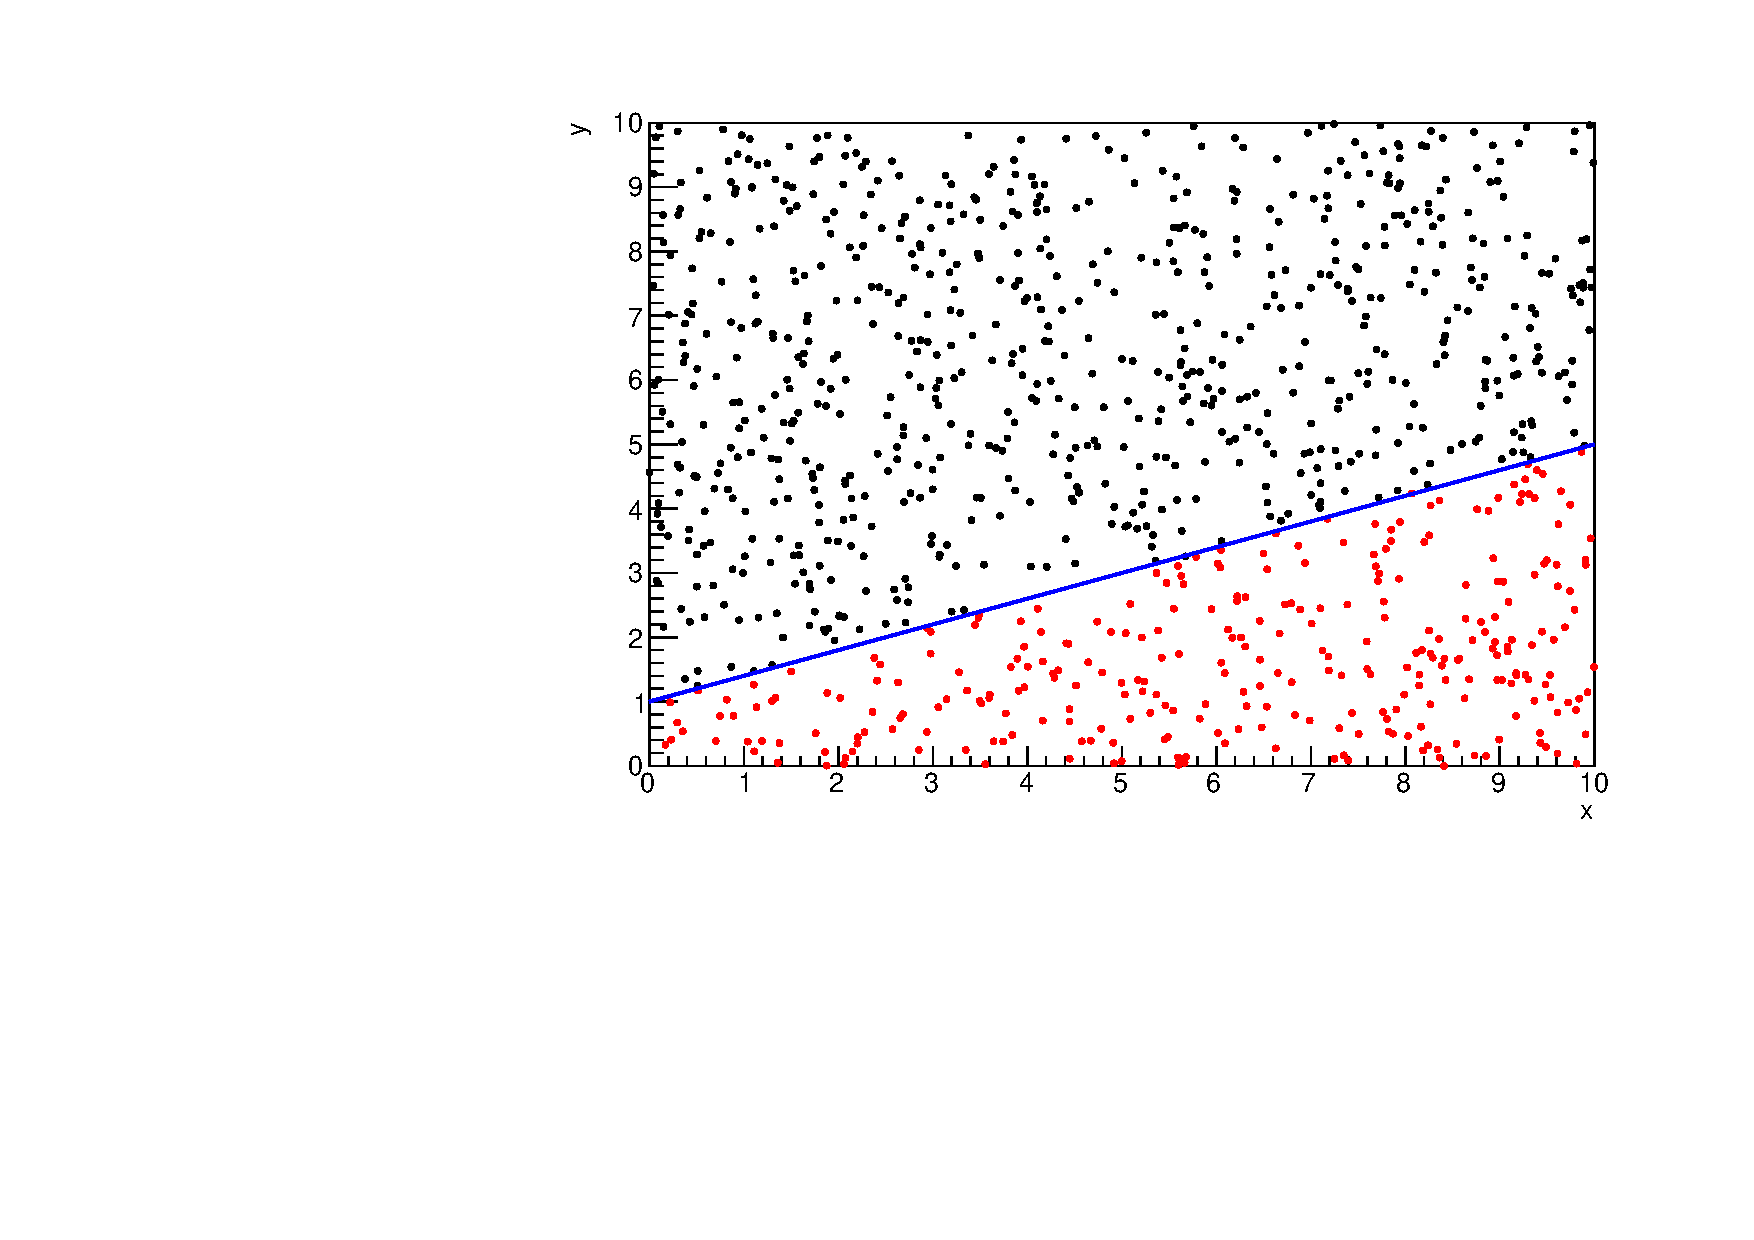
\includegraphics[width=\textwidth, trim={0mm 0mm 0mm 0mm}, clip,page=1]{Figures/MCMC/MCTechnique.pdf}
  \end{subfigure}
  \caption{Example of using Monte Carlo techniques to find the area under the blue line. The gradient and intercept of the line are \quickmath{0.4} and \quickmath{1.0} respectively. The area found to be under the curve using one thousand samples is \quickmath{29.9} units.}
  \label{fig:MCMC_MCTechnique}
\end{figure}

\begin{figure}[h]
  \begin{subfigure}[t]{0.80\textwidth}
    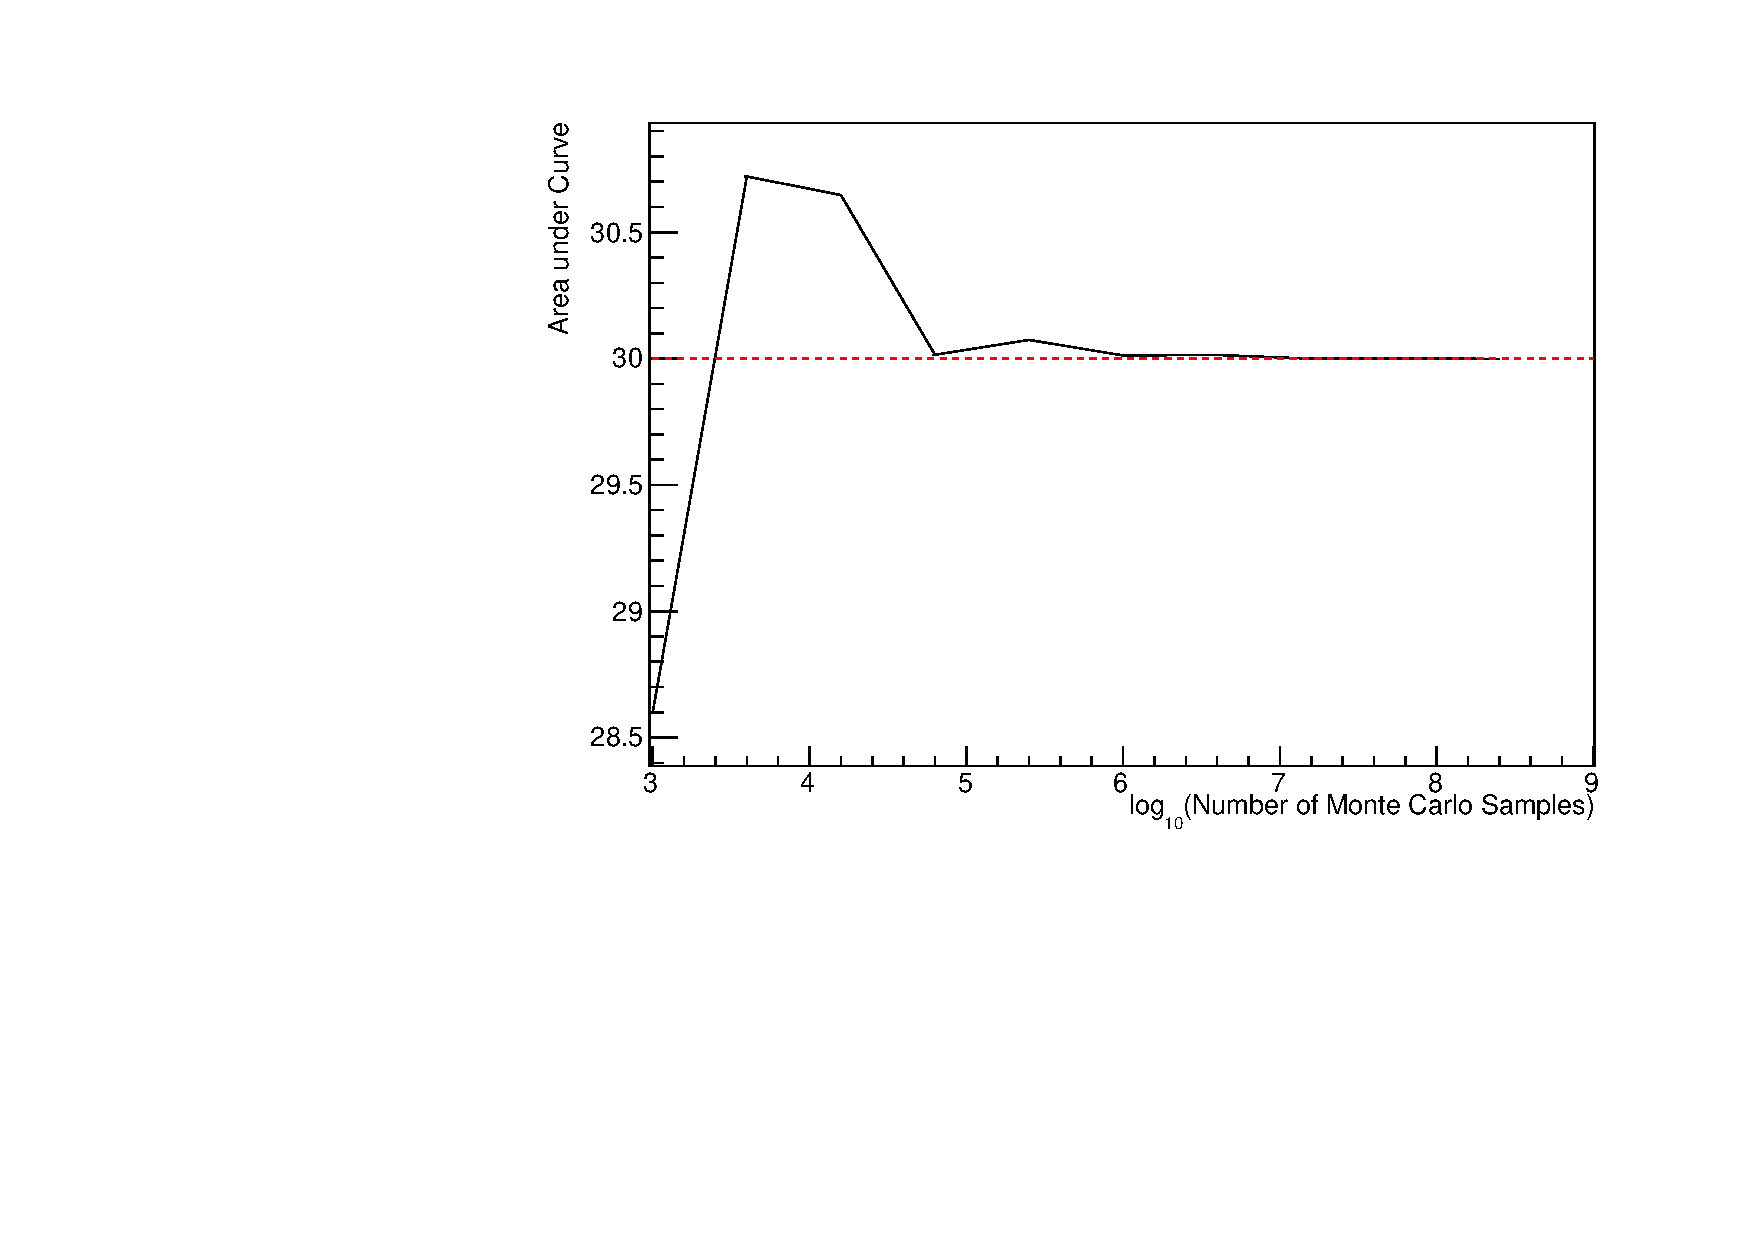
\includegraphics[width=\textwidth, trim={0mm 0mm 0mm 0mm}, clip,page=1]{Figures/MCMC/MCTechnique_NThrowsStudy.pdf}
  \end{subfigure}
  \caption{The area under a line of gradient \quickmath{0.4} and intercept \quickmath{1.0} for the range \quickmath{0 \leq x \leq 10} as calculated using Monte Carlo techniques as a function of the number of samples used in each repetition. The analytical solution to the area is 30 units as given by the red line.}
  \label{fig:MCMC_MCTechniqueNThrowsStudy}
\end{figure}

\subsection{Markov Chain Monte Carlo}
\label{sec:MarkovChainMonteCarlo_MarkovChainMC}
This analysis utilises a multi-dimensional probability distribution, with some dimensions being significantly more constrained than others. This could be from prior knowledge of parameter distributions from external data or un-physical regions in which parameters can not exist. Consequently, the Monte Carlo techniques used need to be as efficient as possible. For this analysis, the Markov Chain Monte Carlo (MCMC) technique is chosen. An MCMC technique is a Monte Carlo technique that uses a Markov chain to select which points at which to sample the parameter distribution. This technique performs a semi-random stochastic walk through the allowable parameter space. This builds a posterior distribution which has the property that the density of sampled points is proportional to the probability density of that parameter. This does mean that the samples produced by this technique are not statistically independent but they will cover the space of the distribution.

A Markov chain functions by selecting the position of step \quickmath{\vec{x}_{i+1}} based on the position of \quickmath{\vec{x}_{i}}. The space in which the Markov chain selects samples is dependent upon the total number of parameters utilised within the fit, where a discrete point in this space is described by the N-dimensional space \quickmath{\vec{x}}. In a perfectly operating Markov chain, the position of the next step depends solely on the previous step and not on the further history of the chain (\quickmath{\vec{x}_{0}}, \quickmath{\vec{x}_{1}}, etc.). However, in solving the multi-dimensionality of the fit used within this analysis, each step becomes correlated with several of the steps preceding itself. This behaviour is further explained in \autoref{sec:MarkovChainMonteCarlo_MCMCOptimisation}. Providing the MCMC chain is well optimised, it will begin to converge towards a unique stationary distribution. The period between the chain's initial starting point and the convergence to the unique stationary distribution is colloquially known as the burn-in period. This is discussed further in \autoref{sec:MarkovChainMonteCarlo_MCMCOptimisation}. Once the chain reaches the stationary distribution, all points sampled after that point will look like samples from that distribution.

Further details of the theories underpinning MCMC techniques are discussed in \cite{mcmc_practice} but can be summarised by the requirement that the chain satisfies the three `regularity conditions':

\begin{itemize}
\item Irreducibility: From every position in the parameter space \quickmath{\vec{x}}, there must exist a non-zero probability for every other position in the parameter space to be reached.
\item Recurrence: Once the chain arrives at the stationary distribution, every step following from that position must be samples from the same stationary distribution.
\item Aperiodicity: The chain must not repeat the same sequence of steps at any point throughout the sampling period.
\end{itemize}

The output of the chain after burn-in (ie. the sampled points after the chain has reached the stationary distribution) can be used to approximate the posterior distribution and model parameters \quickmath{\vec{\theta}}. To achieve the requirement that the unique stationary distribution found by the chain be the posterior distribution, one can use the Metropolis-Hastings algorithm. This guides the stochastic process depending on the likelihood of the current proposed step compared to that of the previous step. Implementation and other details of this technique are discussed in \autoref{sec:MarkovChainMonteCarlo_MetropoliseHastingsAlgorithm}.

\subsection{Metropolis-Hastings Algorithm}
\label{sec:MarkovChainMonteCarlo_MetropoliseHastingsAlgorithm}

As a requirement for MCMCs, the Markov chain implemented in this technique must have a unique stationary distribution that is equivalent to the posterior distribution. To ensure this requirement and that the regularity conditions are met, this analysis utilises the Metropolis-Hastings (MH) algorithm \cite{metropolis, hastings}. For the \quickmath{i^{th}} step in the chain, the MH algorithm determines the position in the parameter space to which the chain moves to based on the current step, \quickmath{\vec{x}_{i}}, and the proposed step, \quickmath{\vec{y}_{i+1}}. The proposed step is randomly selected from some proposal function \quickmath{f(\vec{x}_{i+1}|\vec{x}_{i})}, which depends solely on the current step (ie. not the further history of the chain). The next step in the chain \quickmath{\vec{x}_{i+1}} can be either the current step or the proposed step determined by whether the proposed step is accepted or rejected. To decide if the proposed step is selected, the acceptance probability, \quickmath{\alpha(\vec{x}_{i},\vec{y}_{i})}, is calculated as

\begin{equation}
  \label{eq:MarkovChainMonteCarlo_FullAcceptanceProbability}
  \alpha(\vec{x}_{i},\vec{y}_{i+1}) = \min\left(1,\frac{P(\vec{y}_{i+1}|D)f(\vec{x}_{i}|\vec{y}_{i+1})}{P(\vec{x}_{i}|D)f(\vec{y}_{i+1}|\vec{x}_{i})} \right).
\end{equation}

Where \quickmath{P(\vec{y}_{i+1}|D)} is the posterior distribution as introduced in \autoref{sec:MarkovChainMonteCarlo_BayesianStatistics}. To simplify this calculation, the proposal function is required to be symmetric such that \quickmath{f(\vec{x}_{i}|\vec{y}_{i+1}) = f(\vec{y}_{i+1}|\vec{x}_{i})}. In practice, a multi-variate Gaussian distribution is used to throw parameter proposals from. This reduces \autoref{eq:MarkovChainMonteCarlo_FullAcceptanceProbability} to

\begin{equation}
  \label{eq:MarkovChainMonteCarlo_ReducedAcceptanceProbability}
  \alpha(\vec{x}_{i},\vec{y}_{i+1}) = \min\left(1,\frac{P(\vec{y}_{i+1}|D)}{P(\vec{x}_{i}|D)} \right).
\end{equation}

After calculating this quantity, a random number, \quickmath{\beta}, is generated uniformly between 0 and 1. If \quickmath{\beta \leq \alpha(\vec{x}_{i},\vec{y}_{i+1})}, the proposed step is accepted. Otherwise, the chain sets the next step equal to the current step and this procedure is repeated. This can be interpreted as if the posterior probability of the proposed step is greater than that of the current step, (\quickmath{P(\vec{y}_{i+1}|D) \geq P(\vec{x}_{i}|D)}), the proposed step will always be accepted. If the opposite is true, (\quickmath{P(\vec{y}_{i+1}|D) \leq P(\vec{x}_{i}|D)}), the proposed step will be accepted with probability \quickmath{P(\vec{x}_{i}|D) / P(\vec{y}_{i+1}|D)}. This ensures that the Markov chain does not get trapped in any local minima in the potentially non-Gaussian posterior distribution. The outcome of this technique is that the density of steps taken in a discrete region is directly proportional to the probability density in that region.

\subsection{MCMC Optimisation}
\label{sec:MarkovChainMonteCarlo_MCMCOptimisation}
As discussed in \autoref{sec:MarkovChainMonteCarlo_MetropoliseHastingsAlgorithm}, the proposal function invoked within the MH algorithm can take any form and the chain will still converge to the stationary distribution. At each set of proposed parameter values, a prediction of the same spectra has to be generated which requires significant computational resources. Therefore, the number of steps taken before the unique stationary distribution is found should be minimised as only steps after convergence add information to the oscillation analysis. Furthermore, the chain should entirely cover the allowable parameter space to ensure that all values have been considered. Tuning the distance that the proposal function jumps between steps on a parameter-by-parameter basis can both minimise the length of the burn-in period and ensure that the correlation between step \quickmath{\vec{x}_{i}} and \quickmath{\vec{x}_{j}} is sufficiently small.

The effect of changing the width of the proposal function is highlighted in \autoref{fig:MCMC_MCTechniqueStepSizeStudy}. Three scenarios, each with the same underlying stationary distribution (A Gaussian of width \quickmath{1.0} and mean \quickmath{0.}), are presented. The only difference between the three scenarios is the width of the proposal function, colloquially known as the `step size \quickmath{\sigma}'. Each scenario starts at an initial parameter value of \quickmath{10.0} which would be considered an extreme variation. For the case where \quickmath{\sigma = 0.1}, it is clear to see that the chain takes a long time to reach the expected region of the parameter. This indicates that this chain would have a large burn-in period and does not converge to the stationary distribution until step \quickmath{\sim 500}. Furthermore, whilst the chain does move towards the expected region, each step is significantly correlated with the previous. Considering the case where \quickmath{\sigma = 5.0}, the chain approaches the expected parameter region almost instantly meaning that the burn-in period is not significant. However, there are clearly large regions of steps where the chain does not move. This is likely due to the chain proposing steps in the tails of the distribution which have a low probability of being accepted. Consequently, this chain would take a significant number of steps to fully span the allowable parameter region. For the final scenario, where \quickmath{\sigma = 0.5}, you can see a relatively small burn-in period of approximately \quickmath{100} steps. Once the chain reaches the stationary distribution, it moves throughout the expected region of parameter values many times, sufficiently sampling the full parameter region. This example is a single parameter varying across a continuous distribution and does not fully reflect the difficulties in the many-hundred multi-variate parameter distribution used within this analysis. However, it does give a conceptual idea of the importance of selecting the proposal function and associated step size. 

\begin{figure}[h]
  \begin{subfigure}[t]{\textwidth}
    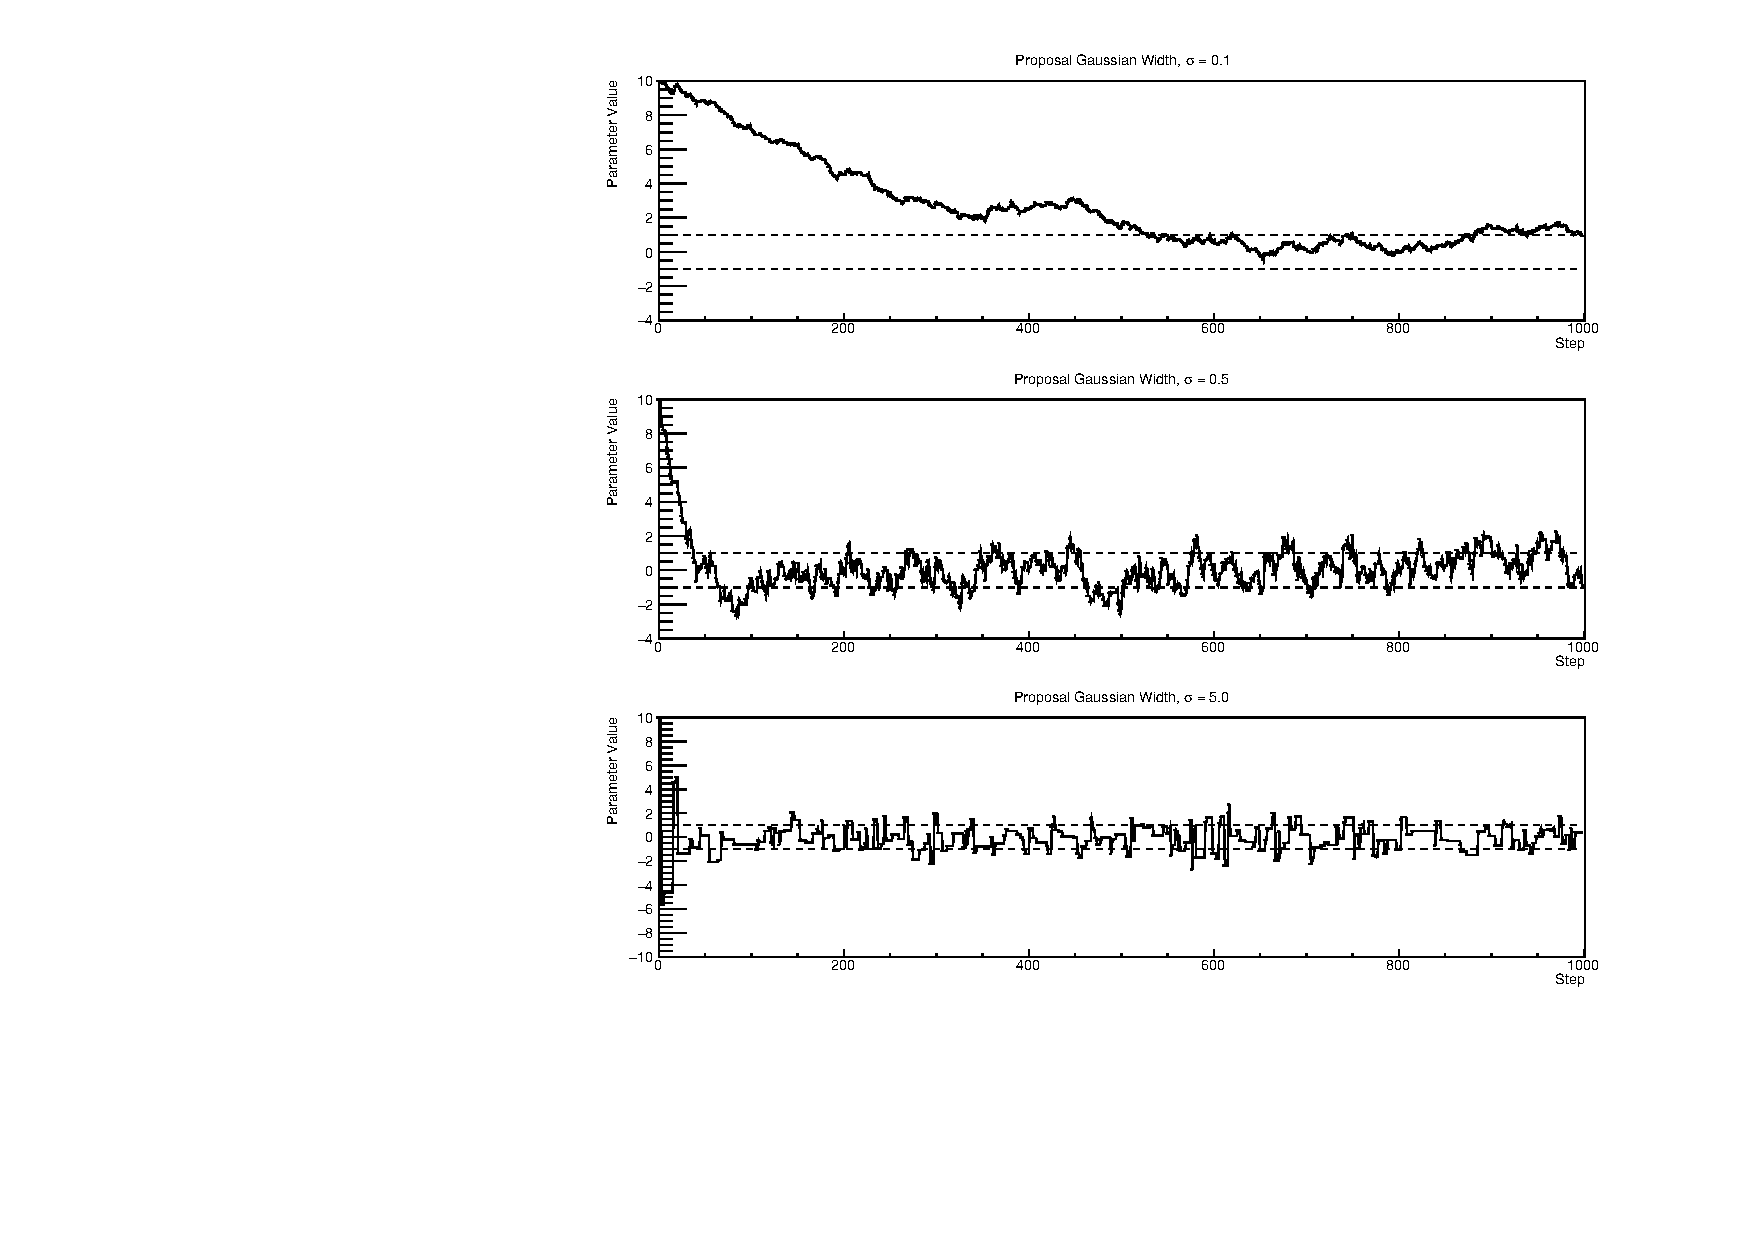
\includegraphics[width=\textwidth, trim={10mm 0mm 18mm 0mm}, clip,page=1]{Figures/MCMC/MCMCTechnique_StepSizes.pdf}
  \end{subfigure}
  \caption{Three MCMC chains, each with a stationary distribution equal to a Gaussian centered at \quickmath{0} and width \quickmath{1} (As indicated by the black dotted lines). All of the chains use a Gaussian proposal function but have different widths (or `step size \quickmath{\sigma}'). The top panel has \quickmath{\sigma = 0.1}, middle panel has \quickmath{\sigma = 0.5} and the bottom panel has \quickmath{\sigma = 5.0}.}
  \label{fig:MCMC_MCTechniqueStepSizeStudy}
\end{figure}

As discussed, step size tuning directly correlates to the average step acceptance rate. If the step size is too small, many steps will be accepted but the chain moves slowly. If the opposite is true, many steps will be rejected as the chain proposes steps in the tails of the distribution. Discussion in \cite{Dunkley2005-xz} suggests that the `ideal' acceptance rate of a high dimension MCMC chain should be approximately \quickmath{\sim 25\%}. An ``ideal'' step size \cite{Dunkley2005-xz} of

\begin{equation}
  \label{eq:MCMC_IdealStepSize}
  \sigma = \frac{2.4}{N_{p}},
\end{equation}

where \quickmath{N_{p}} is the number of parameters included in the MCMC fit. However, the complex correlations between systematics mean that some parameters have to be hand tuned and many efforts have been taken to select a set of parameter-by-parameter step sizes to approximately reach the ideal acceptance rate.

\autoref{fig:MCMC_MCTechniqueStepSizeStudy} highlights the likelihood as calculated by the fit in \finish{Link to AsimovA Sensitivity Section} as a function of the number of steps in each chain. In practice, many independent MCMC chains are run simultaneously to parallelise the task of performing the fit. This figure overlays the distribution found in each chain. As seen, the likelihood decreases from its initial value and converges towards a stationary distribution after \quickmath{\sim 1 \times 10^{5}} steps.

\begin{figure}[h]
  \begin{subfigure}[t]{0.8\textwidth}
    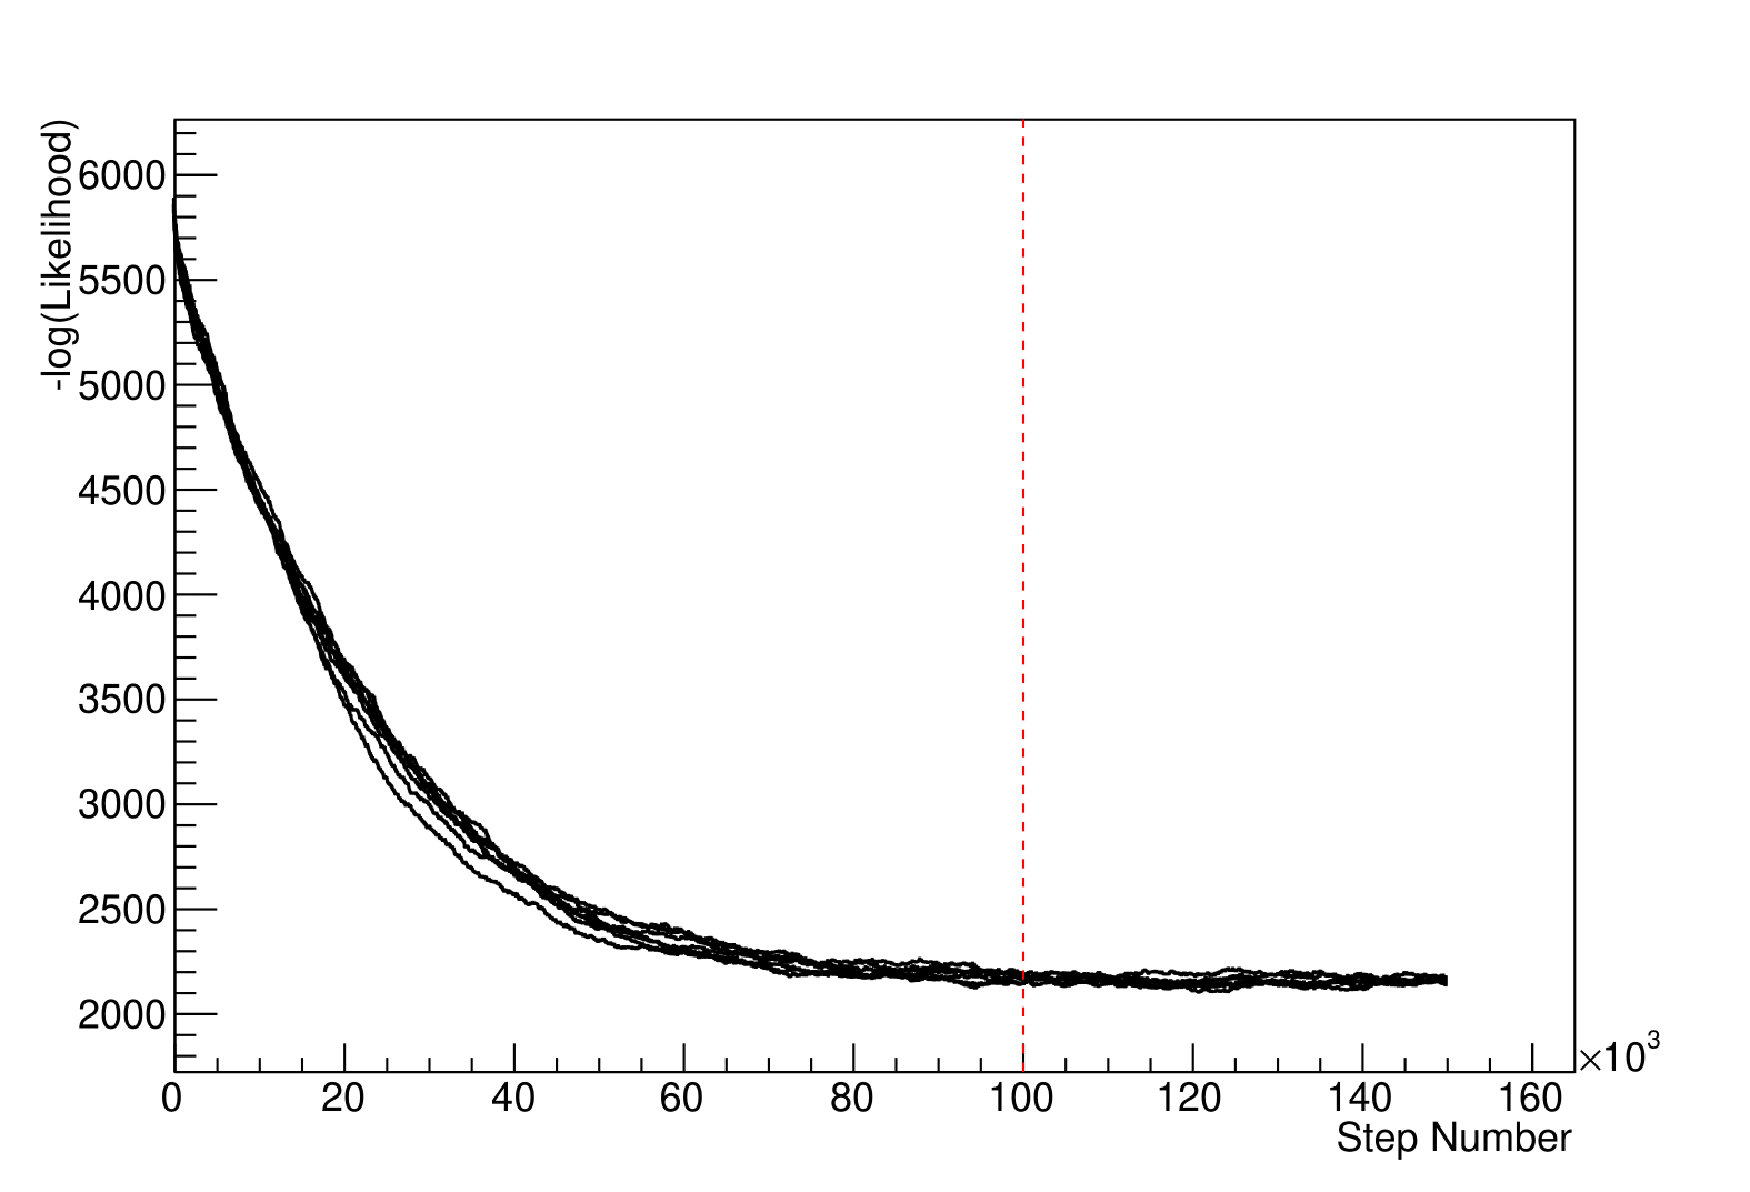
\includegraphics[width=\textwidth, trim={0mm 0mm 0mm 0mm}, clip,page=1]{Figures/MCMC/MCTechnique_LLHStep.pdf}
  \end{subfigure}
  \caption{The log-likelihood from the fit detailed in \finish{Link to AsimovA Sensitivity Section} as a function of the number of steps accumulated in each fit. Many independent MCMC chains were run in parallel and overlaid on this plot. The red line indicates the \quickmath{1 \times 10^{5}} step burn-in period after which the log-likelihood becomes stable.}
  \label{fig:MCMC_MCTechniqueLLHVsStep}
\end{figure}

Multiple configurations of this analysis have been performed throughout this thesis where different samples or systematics have been used. For all of these configurations, it was found that a burnin period of \quickmath{1 \times 10^{5}} was sufficient in all cases.

\section{Understanding the MCMC Results}
\label{sec:MarkovChainMonteCarlo_UnderstandingMCMCResults}

The previous sections have described how to generate the posterior probability distribution using Bayesian MCMC techniques. However, this analysis focuses on oscillation parameter determination. The posterior distribution output from the chain is a high dimension object, with as many dimensions as there are parameters included in the oscillation analysis. However, this multi-dimensional object is difficult to conceptualize so parameter estimations are often presented in one or two-dimensional projections of this probability distribution. To do this, we invoke the marginalisation technique highlighted in \autoref{sec:MarkovChainMonteCarlo_Marginalisation}.

\subsection{Marginalisation}
\label{sec:MarkovChainMonteCarlo_Marginalisation}

The output of the MCMC chain is a highly dimensional probability distribution which is very difficult to interpret. From the standpoint of an oscillation analysis experiment, the one or two-dimensional `projections' of the oscillation parameters of interest are most relevant. Despite this, the best fit values and uncertainties on the oscillation parameters of interest should correctly encapsulate the correlations to the other systematic uncertainties (colloquially called `nuisance' parameters). For this joint beam and atmospheric analysis, the oscillation parameters of interest are \sinsqatm, \sinsqreac, \delmsqatm, and \dcp. All other parameters (Including the oscillation parameter this fit is insensitive to) are deemed nuisance parameters. To generate these projections, we rely upon integrating the posterior distribution over all nuisance parameters. This is called marginalisation. A simple example of this technique is to imagine the scenario where two coins are flipped. To determine the probability that the first coin returned a `head', the exact result of the second coin flip is disregarded and simply integrated over. For the parameters of interest, \quickmath{\vec{\theta}_{i}}, we can calculate the marginalised posterior by integrating over the nuisance parameters, \quickmath{\vec{\theta}_{n}}. In this case, \autoref{eq:MarkovChainMonteCarlo_PosteriorDistribution} becomes

\begin{equation}
P(\vec{\theta}_{i}|D) = \frac{\int P(D|\vec{\theta}_{i},\vec{\theta}_{n}) P(\vec{\theta}_{i},\vec{\theta}_{n}) d\vec{\theta}_{n}}{\int P(D|\vec{\theta}) P(\vec{\theta}) d\vec{\theta}}
\end{equation}

Where \quickmath{P(\vec{\theta}_{i},\vec{\theta}_{n})} encodes the prior knowledge about the uncertainty and correlations between the parameters of interest and the nuisance parameters. In practice, this is simply taking the one or two-dimensional projection of the multi-dimensional probability distribution.

Whilst in principle an easy solution to a complex problem, correlations between the interesting and nuisance parameters can bias the marginalised results. A similar effect is found when the parameters being marginalised over have non-Gaussian probability distributions. For example, \autoref{fig:MCMC_MCTechniqueMarginalisationProblems} highlights the marginalisation bias in the probability distribution found for a parameter when requiring a correlated parameter to have a positive parameter value. Due to the complex nature of this oscillation parameter fit presented in this thesis, there are correlations occurring between the oscillation parameters of interest and the other nuisance parameters included in the fit.

\begin{figure}[h]
  \begin{subfigure}[t]{0.48\textwidth}
    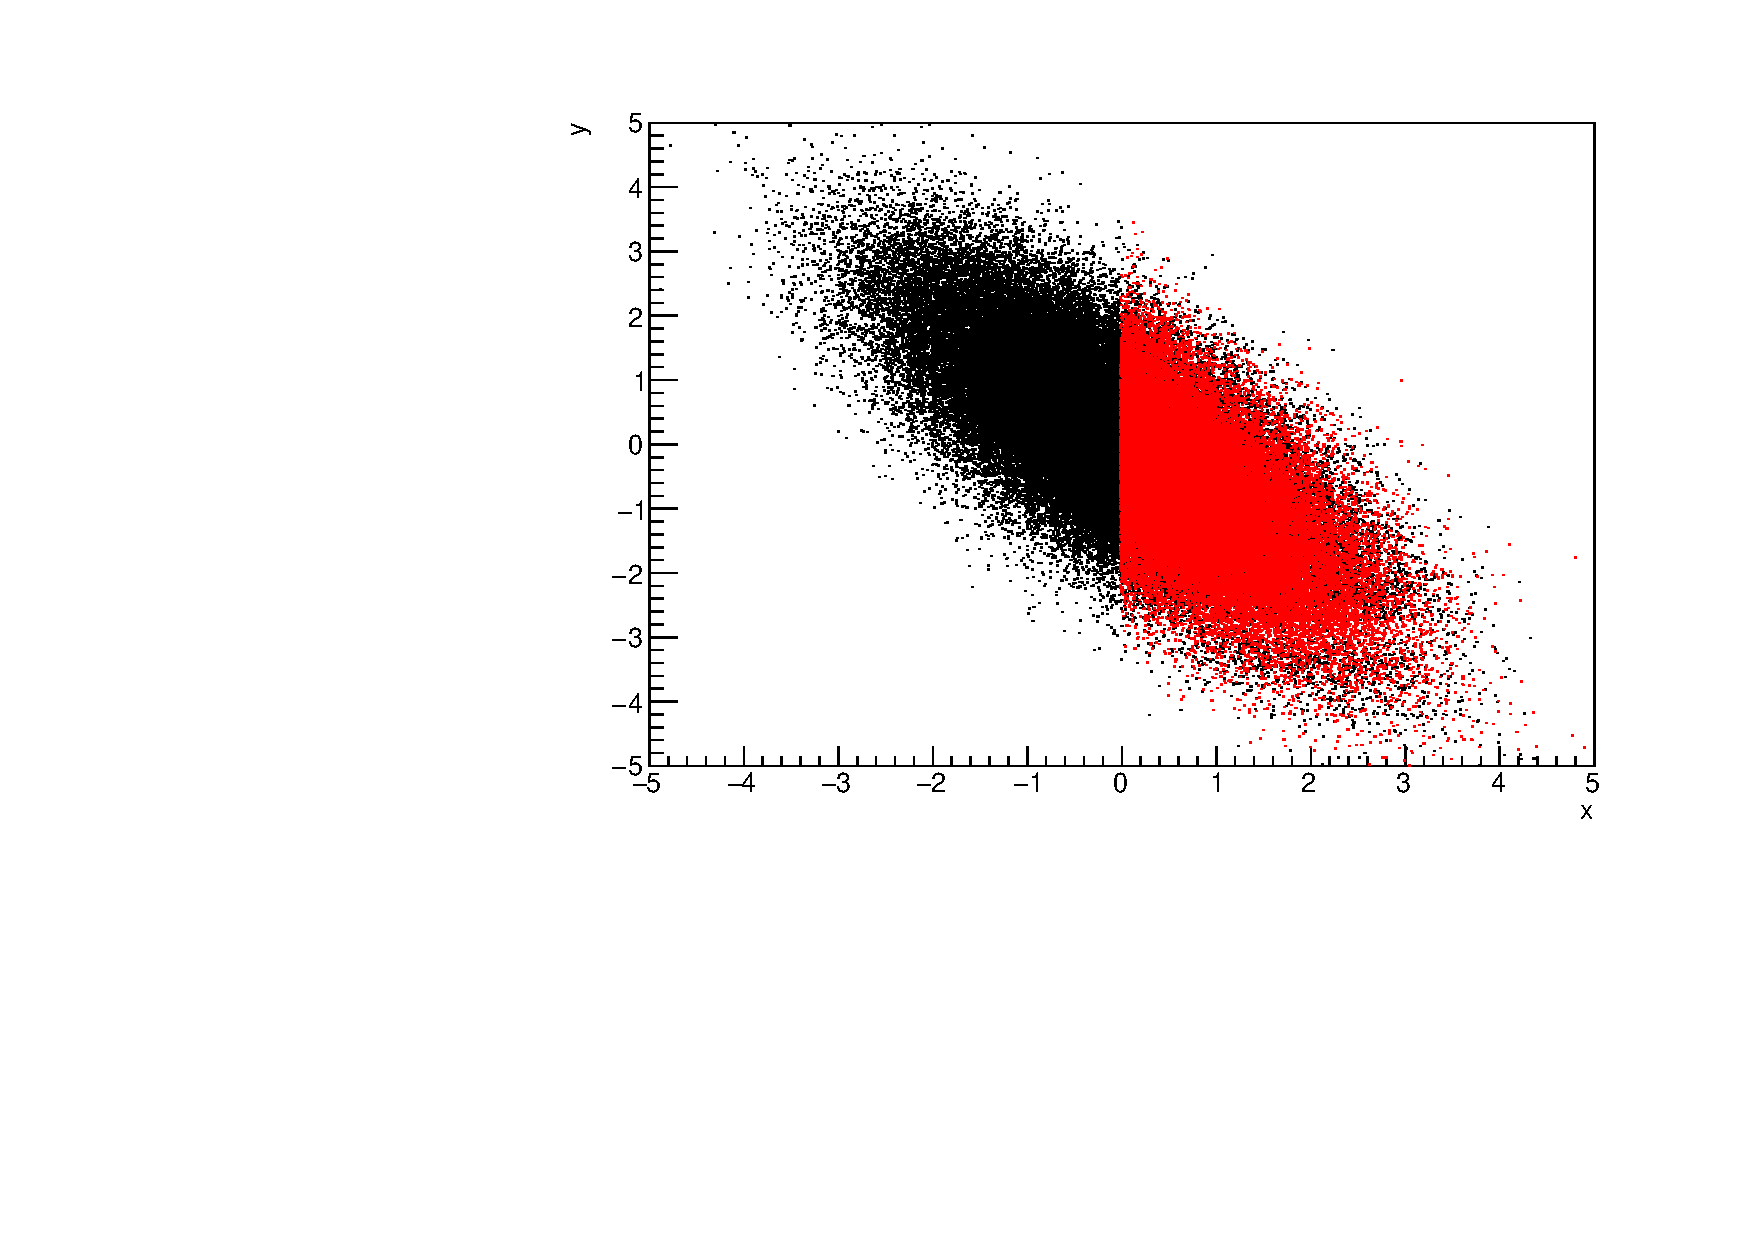
\includegraphics[width=\textwidth, trim={0mm 0mm 0mm 0mm}, clip,page=1]{Figures/MCMC/MCTechnique_Marginalisation2D_Double_Correlations.pdf}
  \end{subfigure} %
    \begin{subfigure}[t]{0.48\textwidth}
    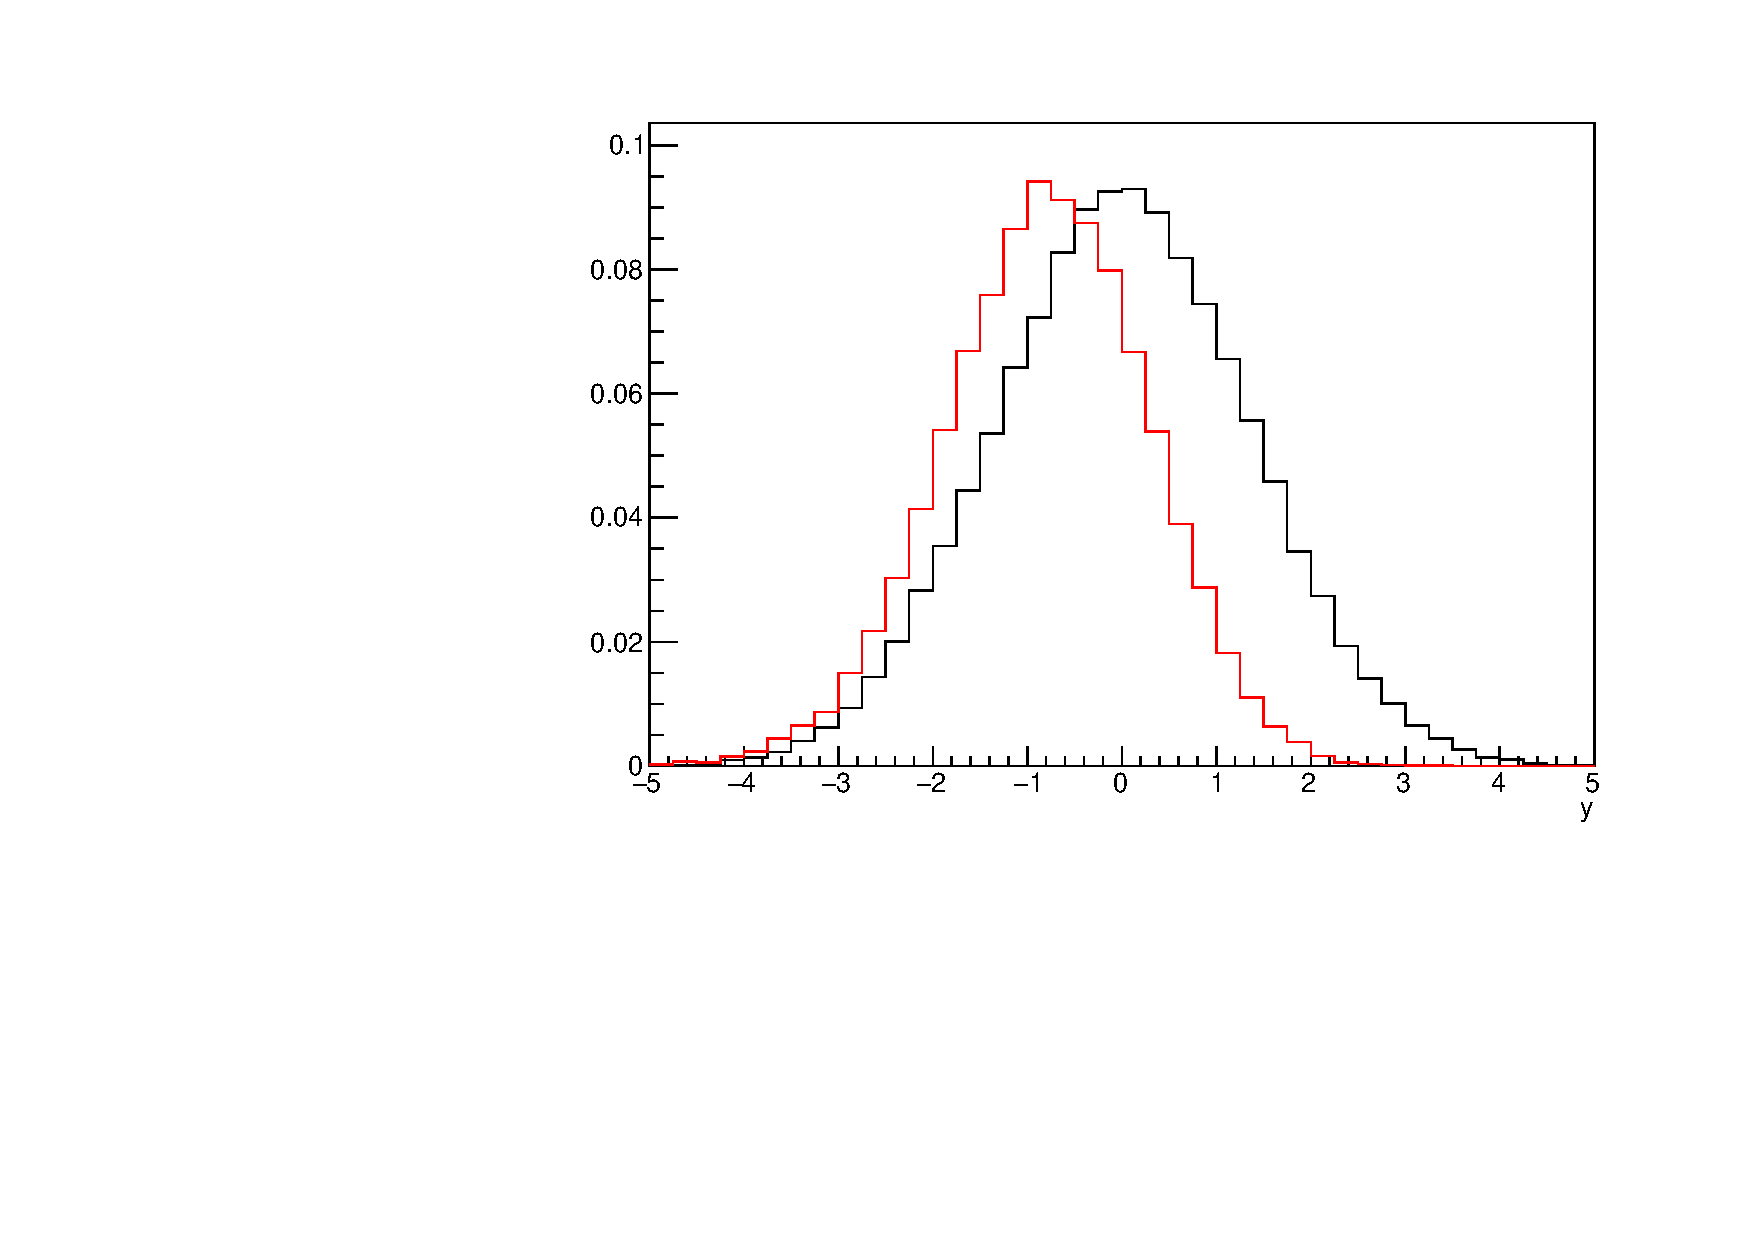
\includegraphics[width=\textwidth, trim={0mm 0mm 0mm 0mm}, clip,page=1]{Figures/MCMC/MCTechnique_Marginalisation1D_Double_Correlations.pdf}
  \end{subfigure}

  \caption{Left: The two dimensional probability distribution for two correlated parameters \quickmath{x} and \quickmath{y}. The red distribution shows the two dimensional probability distribution when \quickmath{0 \leq x \leq 5}. Right: The marginalised probability distribution for the \quickmath{y} parameter found when requiring the \quickmath{x} to be bound between \quickmath{-5 \leq x \leq 5} and \quickmath{0 \leq x \leq 5} for the black and red distribution, respectively.}
  \label{fig:MCMC_MCTechniqueMarginalisationProblems}
\end{figure}

\subsection{Parameter Estimation and Credible Intervals}
\label{sec:MarkovChainMonteCarlo_ParameterEstimation}

The purpose of this analysis is to determine the best fit values for the oscillation parameters that the beam and atmospheric samples are sensitive to: \sinsqatm, \sinsqreac, \delmsqatm, and \dcp. Typically, the results presented take the form of one or two-dimension marginalised probability distributions for the appearance (\sinsqreac and \dcp) and disappearance (\sinsqatm and \delmsqatm) parameters. The posterior probability density taken from the output MCMC chain is binned in these parameters. The parameter best-fit point is then taken to be the value that has the highest posterior probability. This is performed in both one and two-dimensional projections.

However, the single best-fit point in a given parameter is not of much use on its own. We would also like to determine the uncertainty, or credible interval, on that best-fit point. The definition of the \quickmath{1\sigma} credible interval is that we have \quickmath{68\%} belief that the parameter is within those bounds. For a more generalised definition, the credible interval is the region, \quickmath{R}, of the posterior distribution that contains a specific fraction of the total probability, such that

\begin{equation}
\int_{R} P(\theta|D)d\theta = \alpha
\end{equation}

Where \quickmath{\theta} is the parameter on which we calculate the credible interval. This technique then calculates the \quickmath{\alpha \times 100\%} credible interval.

In practice, this analysis uses the highest posterior density (HPD) credible intervals which are calculated through the following method. First, the probability distribution is area-normalised such that it has an integrated area equal to \quickmath{1.0}. The bins of probability are then summed from the highest to lowest until the sum exceeds the \quickmath{1\sigma} level (\quickmath{0.68} in this example). This process is repeated for a range of credible intervals, notably the \quickmath{1\sigma}, \quickmath{2\sigma} and \quickmath{3\sigma} along with other levels where the critical values for each level can be found in \cite{Particle_Data_Group2020-ms}. This process can be repeated for the two-dimensional probability distributions by creating two-dimensional contours of credible intervals rather than a one-dimensional result. 

\subsection{Bayesian Model Comparisons}
\label{sec:MarkovChainMonteCarlo_BayesTheorem}
Due to the matter resonance, this analysis has some sensitivity to the mass hierarchy of neutrino states (whether \delmsqatm is positive or negative) and the octant of \sinsqatm. The Bayesian approach utilised within this analysis gives an intuitive method of model comparison by determining which hypothesis is most favourable. Taking the ratio of \autoref{eq:MarkovChainMonteCarlo_PosteriorDistributionReduced} for the two hypotheses of normal hierarchy, \quickmath{NH}, and inverted hierarchy, \quickmath{IH}, gives

\begin{equation}
  \frac{P(\vec{\theta}_{NH}|D)}{P(\vec{\theta}_{IH}|D)} = \frac{P(D|\vec{\theta}_{NH})}{P(D|\vec{\theta}_{IH})} \times \frac{P(\vec{\theta}_{NH})}{P(\vec{\theta}_{IH})}.
\end{equation}

The middle term defines the Bayes factor which is a data-driven interpretation of how strong the data prefers one hierarchy to the other. For this analysis, equal priors on both mass hierarchy hypotheses are chosen (\quickmath{P(\vec{\theta}_{NH}) = P(\vec{\theta}_{IH})} = 0.5). In practice, the MCMC chain proposes a value of \quickmath{|}\delmsqatm\quickmath{|} and then applies a \quickmath{50\%} probability that the value is sign flipped. Consequently, the Bayes factor can be calculated from the ratio of the probability density in either hypothesis. This equates to counting the number of steps taken in the normal and inverted hierarchies and taking the ratio. The same approach can be taken to compare the upper octant (UO) compared to the lower octant (LO) hypothesis of \sinsqatm.

Whilst the value of the Bayes factor should always be shown, the Jeffreys scale \cite{Jeffreys:1939xee} (highlighted in \autoref{tab:MarkovChainMonteCarlo_JeffreysScale}) gives an indication of the strength of preference for one model compared to the other. Other interpretations of the strength of preference of a model exist, e.g. the Kass and Raferty Scale \cite{Kass1995-nl}.

\begin{table}[ht!]
    \centering
    \begin{tabular}{c|c|l}
      \hline
      $\log_{10}(B_{AB})$ & $B_{AB}$ & Strength of Preference \\
      \hline
      \hline
      \quickmath{<0.0} & \quickmath{<1} & No preference for hypothesis A (Supports hypothesis B) \\
      \quickmath{0.0 - 0.5} & \quickmath{1.0 - 3.16} & Preference for hypothesis A is weak \\
      \quickmath{0.5 - 1.0} & \quickmath{3.16 - 10.0} & Preference for hypothesis A is substantial \\
      \quickmath{1.0 - 1.5} & \quickmath{10.0 - 31.6} & Preference for hypothesis A is strong \\
      \quickmath{1.5 - 2.0} & \quickmath{31.6 - 100.0} & Preference for hypothesis A is very strong \\
      \quickmath{>2.0 }& \quickmath{>100.0} & Decisive preference for hypothesis A \\
      \hline
      \hline
      
      \hline
    \end{tabular}
    \caption{Jeffreys scale for strength of preference for two models \quickmath{A} and \quickmath{B} as a function of the calculated Bayes factor (\quickmath{B_{AB} = B(A/B)}) between the two models \cite{Jeffreys:1939xee}. The original scale is given in terms of \quickmath{\log_{10}(B(A/B))} but converted to linear scale for easy comparison throughout this thesis.}
    \label{tab:MarkovChainMonteCarlo_JeffreysScale}
\end{table}

\subsection{Comparison of MCMC Output to Expectation}
\label{sec:MarkovChainMonteCarlo_Predictives}

To ensure the fit is performing well, a best-fit spectrum is produced using the posterior probability distribution and compared with the data, allowing easy by-eye comparisons to be made. A simple method of doing this is to perform a comparison in the fitting parameters (For instance, the reconstructed neutrino energy and lepton direction for T2K far detector beam samples) of the spectra generated by the MCMC chain to `data'. This `data' could be true data or some variation of Monte Carlo prediction. This allows easy comparison of the MCMC probability distribution to the data. To perform this, \quickmath{N} steps from the post burn-in MCMC chain are randomly selected (Where for all plots of this style in this thesis, \quickmath{N=3000}). From these, the Monte Carlo prediction at each step is generated by reweighting the model parameters to the values specified at that step. Due to the probability density being directly correlated with the density of steps in a certain region, parameter values close to the best fit value are most likely to be selected.

In practice, for each bin of the fitting parameters has a probability distribution of event rates, with one entry per sampled MCMC step. This distribution is binned where the bin with the highest probability is selected as the mean and an error on the width of this probability distribution is calculated using the approach highlighted in \autoref{sec:MarkovChainMonteCarlo_ParameterEstimation}. Consequently, the best fit distribution in the fit parameter is not necessarily that which would be attained by reweighting the Monte Carlo prediction to the most probable parameter values.

A similar study can be performed to illustrate the freedom of the model parameter space prior to the fit. This can be done by throwing parameter values from the prior uncertainty of each parameter. This becomes troublesome for parameters with no prior uncertainty as the range is technically infinite. Where applicable solutions to remove these have been addressed.
